\chapter{Основная часть}
\section{Имеющиеся данные}
В рамках программы SAHR были записаны ЭКГ (использовалось только первое отведение) 1800 москвичей преклонного возраста (55-91 год). Из них 46\% мужчин. 81\% из них чувствовал себя во время обследования хорошо, 19\% - плохо. 49\% имеют высшее образование. Также имеются данные об общем состоянии физического и психического здоровья каждого человека, индекс массы тела и множество других данных о его состоянии (заболевание, курит ли человек, с какого возраста и т.п.) Запись каждого ЭКГ производилась с помощью холтеров в течение суток. В это же время за человеком велось дополнительное наблюдение и было известно, в какой промежуток времени он спал, а в какой - бодрствовал.
\section{Постановка задачи}

Цель работы - анализируя данные ЭКГ предсказать в какое время человек спал/бодроствовал, исследовать возможность предсказания болезней и самочувствия человека.Также в рамках обучени выделения признаков и их анализа были проведены исследования по идентификации человека.

\section{Актуальность задачи}
Электрокардиография - самый распространенный клинический инструмент, который измеряет электрическую деятельность сердца с поверхности тела. Сигнал ЭКГ, или проще вариабельности сердечного ритма содержит много интересной информации о человеке. Сейчас медицинские институты в дополнение к существующим базам данных (SAHR, AHA DB, ESC DB и т. д.) формируют новые. Также разработано множество новых технологий и приборов, таких как фитнесс-браслеты, специальные чехлы для телефонов, мониторы-холтеры и др., позволяющих человека без каких либо трудностей и специального медицинского оборудования круглосуточно (или в любое удобное для него время) записывать информацию о своем пульсе. Для врачей повилась возможность постоянно контролировать состояние пациента и отправлять их данные  для анализа и отчетности. Популярность подобных носимых устройств для мониторинга здоровья растет с каждым годом. Они позволяют человеку быть подвижным, заниматься своими делами и в это же время собирать данные о своем здоровье в "естественной" среде. Точность этих приборов уступает специализированным установкам - но даже по их сигналу можно многое сказать о человеке. 

Качество и длительность сна имеют важное значение для медицинской диагностики []. Однако на практике сложность процедуры классической полисомнографии [] накладывает существенные ограничения для ее применения. Несмотря на множество информации, которую предоставляют носимые электронные устройства и исслдеований в этом направлении, на сегодняшний день нет хороших научных доказательств, представленных публике, о том, что они могут оценить продолжительность сна с высокой точностью.

\section{Фильтрация ЭКГ сигнала и выделение RR-пиков}
\subsection{Фильтрация ЭКГ}
Сигнал ЭКГ, собираемый носимыми устройствами, подвержен влиянию множества шумов. На него могут влият следующие причины, никак напрямую не связанные с сердцем.
\begin{itemize}
	\item Погрешности устройства
	\item Неплотное прилегание устройства к коже
	\item Подвижность человека (сокращения мыщц, и др.)
	\item Физические реакции, не связанные с рердечной деятельность (к примеру, внезапные сокращения мыщц при засыпании)
\end{itemize}
%Иногда сигнал с устройства выглядит следующим образом. рис.

\subsection{Выделение RR-пиков}
Для определения R-пиков данный сигнал обрабатывался рядом фильтров. На первом этапе нам наиболее важно выделить найти местоположение R-пиков и не имеет значения, какой вид примет QRS-комплекс. Фильтрация производится на основе дискретного преобразования Фурье (ДПФ): проводится ДПФ, зануляются нужные коэффициенты и производится обратное преобразование ДПФ. Какие именно коэффициенты занулять «подсмотрено» в сторонних библиотеках Matlab для анализа кардиограмм.

Вид сигнала после применения фильтров можно наблюдать на рис.  \ref{ris:filter_ekg}

\begin{figure}[h]
	\begin{minipage}[h]{0.47\linewidth}
		\center{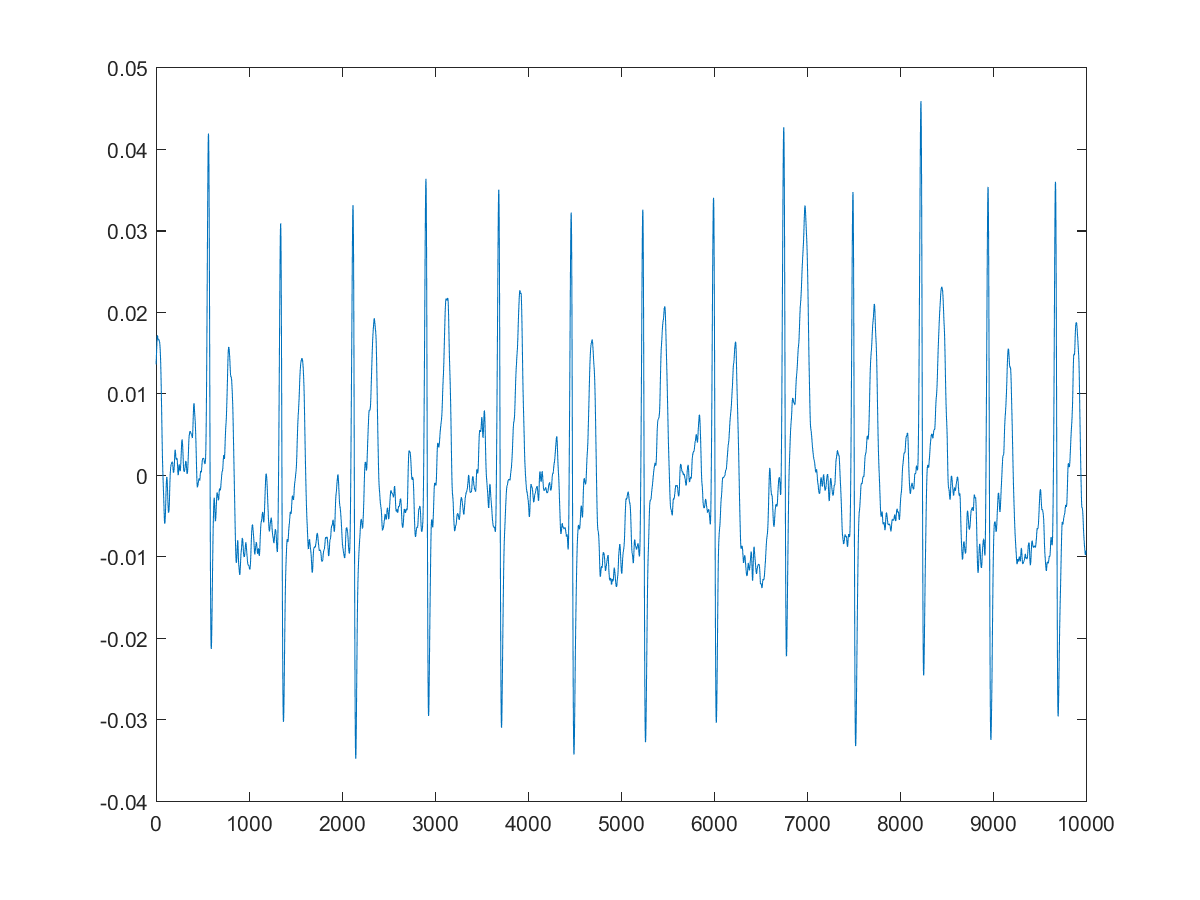
\includegraphics[width=1\linewidth]{filtered_ekg_base}} a) \\
	\end{minipage}
	\hfill
	\begin{minipage}[h]{0.47\linewidth}
		\center{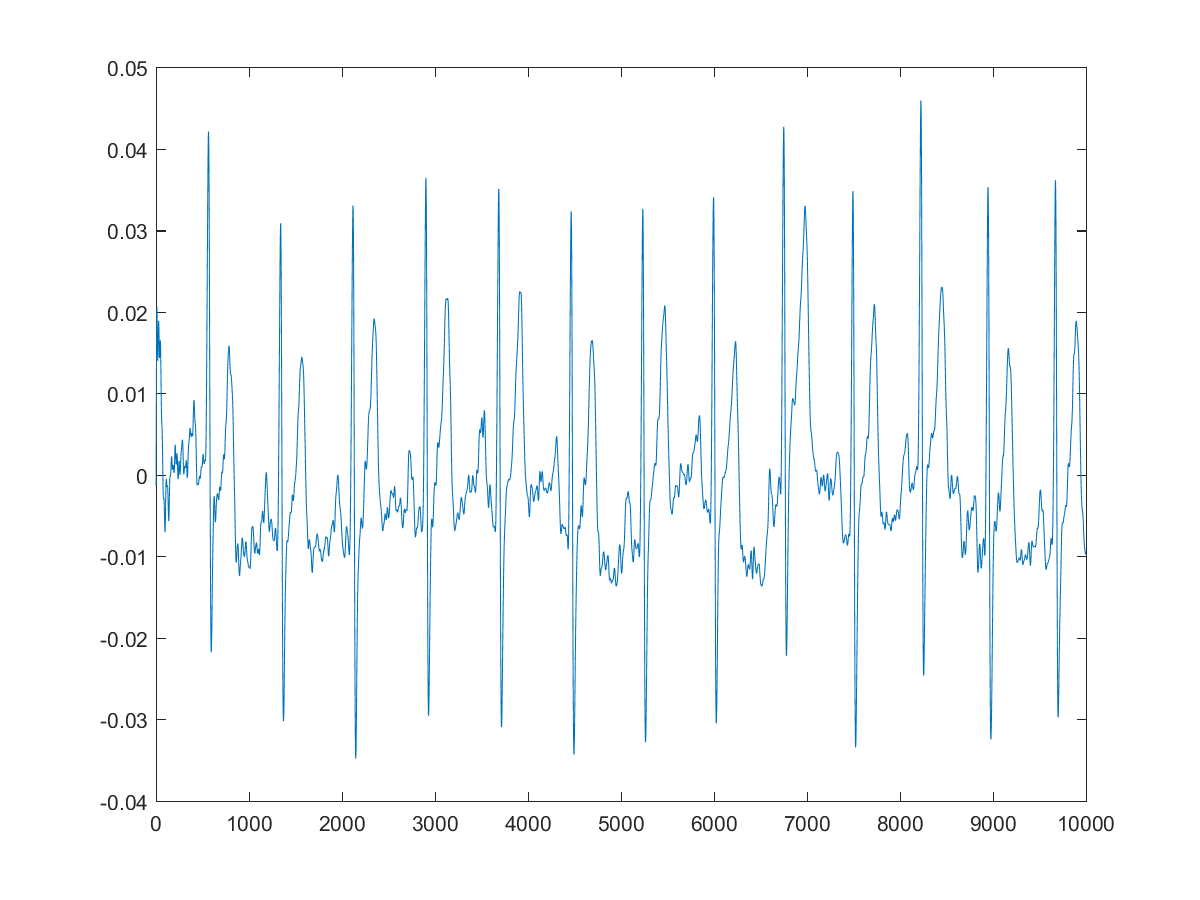
\includegraphics[width=1\linewidth]{filtered_ekg_hig}} \\b)
	\end{minipage}
	\vfill
	\begin{minipage}[h]{0.47\linewidth}
		\center{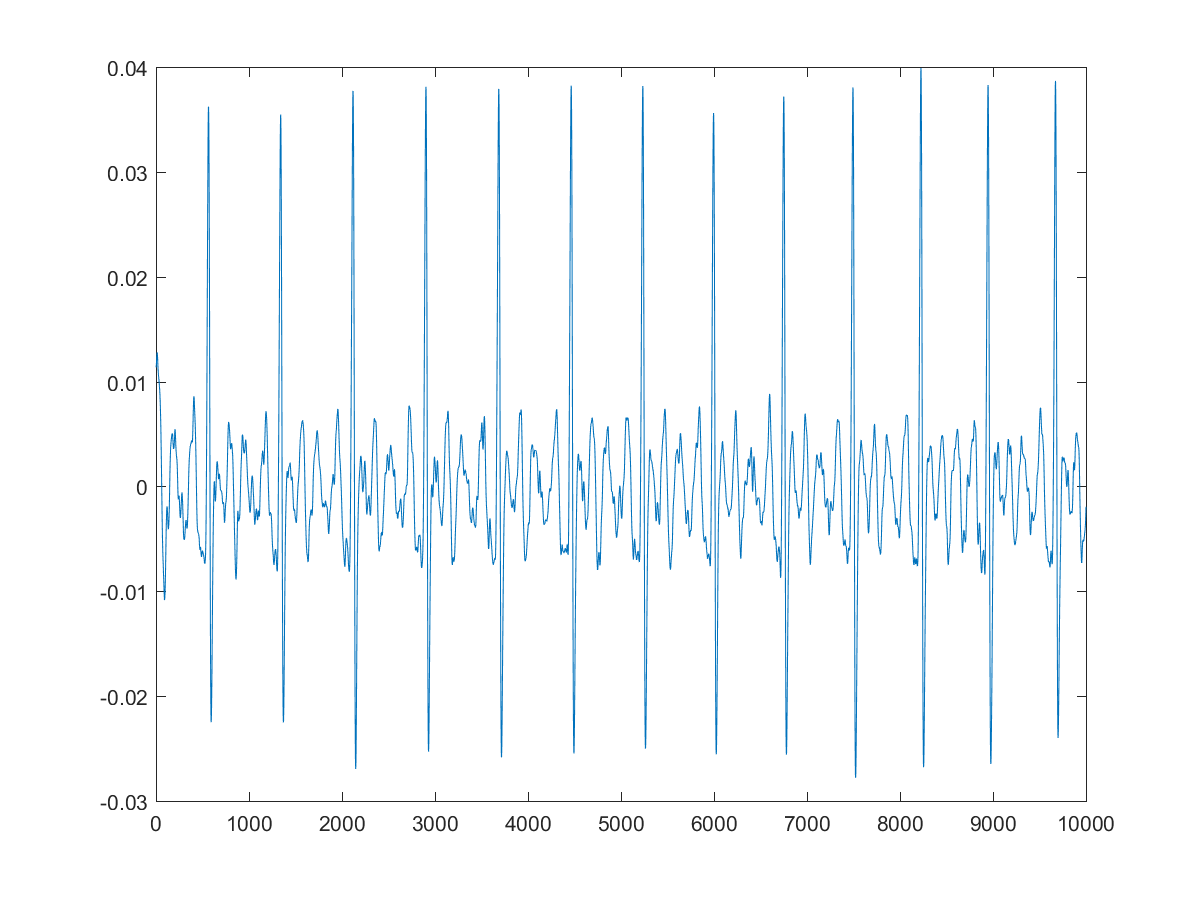
\includegraphics[width=1\linewidth]{filtered_ekg_low}} c) \\
	\end{minipage}
	\hfill
	\begin{minipage}[h]{0.47\linewidth}
		\center{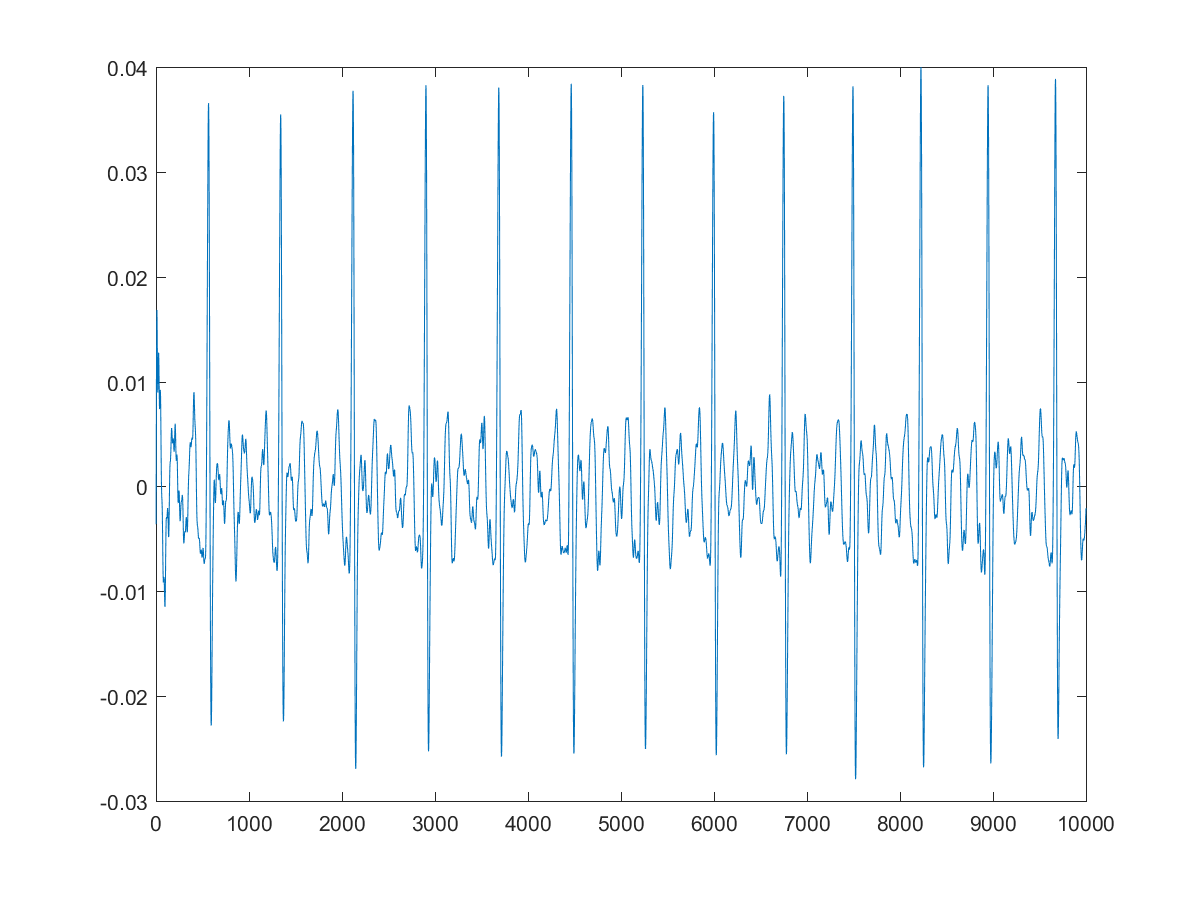
\includegraphics[width=1\linewidth]{filtered_ekg_low_hig}} d) \\
	\end{minipage}
	\caption{ЭКГ сигнал a)до фильтрации b) после высокочастотного фильтра
		c) после низкочастотного фильтра d) после обоих фильтров}
	\label{ris:filter_ekg}
\end{figure}

Для определения RR-пиков отбирались точки $i$ такие, что $x_i$ - локальный максимум в окне $[x_{i-k\_pred}, ..., x_i,    , x_{i+k\_next}]$, а также $min([x_{i-r\_pred}, ..., x_i])<0$ и $min([x_i, ..., x_{i+r\_next}])<0$. То есть сигнал справа и слева от локального минимума опускается ниже нуля. Напомню, что мы работаем с фильтрованным сигналом, среднее значение которого лежит около нуля.

Далее, когда мы определили координаты пиков на фильтрованном сигнале - находим обратным преобразванием их на исходном. Признаки, считаемые по QRS-комплексу считались по неотфильтрованныму сигналу, дабы не потерять информацию. Фильтр низких частот, применение которого желательно при поиске пиков, очень сильно искажает сигнал. 
QRS-комплекс размечался по следующему алгоритму:
статья дьяконова
код никиты - ссылки из него
картинки найденного QRS-комлекса

\section{Работа с RR-сигналом}
\subsection{Отбор RR-пиков}
При снятии сигнала возникают лишние пики. Они могут быть вызваны сокращениями мыщц, резкими движениями или другими различными причинами. При не очень плотном прилегании электрода какой-то кусок сигнала может быть потерян. При первичной обработке сигнала вырезались длительные участки сигнала без пиков (если на протяжени 2 минут не было пиков), и выкидывался участок сигнала между пиками, расположенными ближе чем 200 мс.

примеры плохого сигнала

Для классификации промежутков времени на сон/бодрствование необходим весь временной ряд. Но для идентификации человека, для предсказания каких-либо характеристик достаточно только его части. Если брать для предсказания характеристик небольшие участки сигнала размер обучающей выборки увеличится в несколько раз, увеличится ее обобщающая способность.

То, что мы берем только участки сигнала позволяет нам отобрать участки с минимумом шума. На сигнал могут влиять случайные движения человека, непроизвольные сокращения мыщц. Может быть не очень хорошо закреплен электрод или же он может сдвинуться или отойти на время. в первом случае мы получаем лишние пики, во втором, наоборот, долгий промежуток без них. 

Было решено отбирать участки сигнала где все выделенные R-пики удовлетворяют следующим условиям:

\begin{itemize}
	\item разница высот соседних пиков менее 20\%
	\item разница продолжительностей соседних RR интервалов менее 20\%
\end{itemize}

\subsection{Выделение признаков}
Большая часть подсчитываемых признаков по выделенным R пикам описана в обзоре литературы - они являются стандартными при работе в ЭКГ сигналом. Однако вдобавок к ним использовались еще добавочные признаки.
\begin{itemize}
	\item амплитуды пиком и минимумов в QRST-комплексе
	\item разница высот между пиками P, R, T
	\item отношения ввысот P, R, T
	\item средние значения на промежутках PQ, QR, QT
	\item длительнисть различных фаз в QRST-комплексе
	\item площадь под графиком на промеежутках PQ, QS, ST, begin-Q, S-final
\end{itemize}
В медицине утверждается [!! ссыдки], что врачи ориентируются на данные параметры при постановки диагноза.
\section{Проведенные экперименты}

В рамках данного исследовая проводились попытки решения следующих задач.
\subsection{Идентификация человека}
Люди делились на 3 выборки: тестовую, валидационную и обучающую. Экг каждого человека нарезались на отрезки. Состовлялись пары отрезков, для каждой пары устанавливалось из одного сигнала они взяты (1) или из разных (0). Далее пары отрезков подавались на вход сети :
 архитектуру? надо ли вообще. я об этом так себе знаю - это твое исследование было
Качество предсказания на тестовом датасете - 75\%. Количество элементов каждого класса во всех выборках было равным.
\subsection{Предсказание сна}
Перед нами стояла задача по заданному RR-сигналу определить периоды сна и бодрствования для каждого человека. Данная задача представляет интерес, так как продолжительность сна является важным маркером здоровья.

При анализе сигнал разбивался на части определенной длины и для каждого полученного промежутка определялось состояние человека (спит или бодрствует). 

Необходимо помнить, что при решении данной задачи всегда будет присутствовать определенная погрешность. Процесс погружения в сон не моментален и обычно занимает некоторый промежуток времени.

Важно выбрать не слишком короткий и не слишком длинный промежуток времени для анализа. Если он будет коротким, на него будут сильно влиять различные мгновенные причины (такие как случайные движения, непроизвольные сокращения мышц и др.), не имеющие отношения к серцебиению и состоянию организма. Он не должен быть слишком длинным - чем длиннее данный промежуток, тем больше погрешность определения границ сна. При анализе достаточно длительного промежутка могут быть потеряны различные высокочастотные особенности, которые будут усреднены. Оптимальным по длительности был признан промежуток в 5 минут.
В ходе данного исследования эта задача решалась следующими методами.
\subsubsection{Линейный классификатор}
Если смотреть на RR-сигнал во время сна и бодроствования (одну картинку сюда - сделать красиво) можно заметить, что во время сна частота пульса уменьшается (достаточно очевидное ,предположение известное всем). Также можно заметить уменьшение дисперсия сигнала во время сна.
Первым предложенным алгоритмом был следующий.
\begin{enumerate}
	\item для каждых 200 отсчетов сигнала подсчитывались среднее значение. далее мы работает с последовательностью средних и определяем границе с погрешностью в 100 отсчетов (половина цены деления)
	\item маркируются все точки сигнала на три категории
	\begin{itemize}
		\item точки больше среднего значения ($if mean_i > mean(all\ signal\ mean)$))
		\item точки на половину дисперсии меньше среднего значения ($if mean_i < mean(all\ signal\ mean) - 0.5*std(all\ signal\ mean)$) )
		\item все остальные точки
	\end{itemize}
	\item Далее мы ищем наиболее длинную последовательность точек из первой группы, начинающуюся со 100 не прерываемых точек, не прерываемую более чем 5 точками из второй в любом последующем ее месте. Помним, что в данном контексте точка - это среднее двухсот отсчетов RR-сигнала.
\end{enumerate}
Средняя ошибка предсказания границ ~ час.
На 80\% тестовой выборки абсолютная составляла менее 30 минут.
\begin{figure}[h]
	\begin{minipage}[h]{0.47\linewidth}
		\center{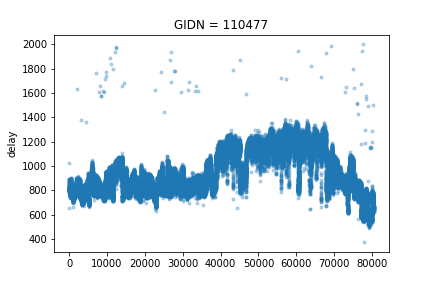
\includegraphics[width=1\linewidth]{1104770}} a) \\
	\end{minipage}
	\hfill
	\begin{minipage}[h]{0.47\linewidth}
		\center{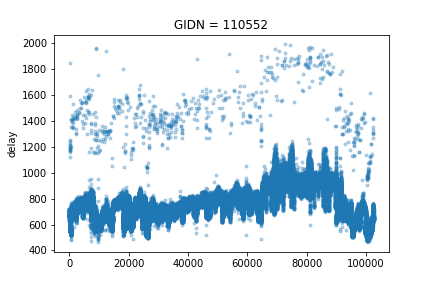
\includegraphics[width=1\linewidth]{1105520}} \\b)
	\end{minipage}
	\vfill
	\begin{minipage}[h]{0.47\linewidth}
		\center{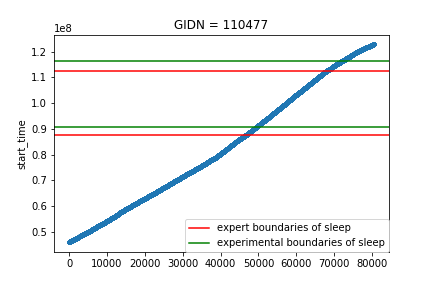
\includegraphics[width=1\linewidth]{1104771}} c) \\
	\end{minipage}
	\hfill
	\begin{minipage}[h]{0.47\linewidth}
		\center{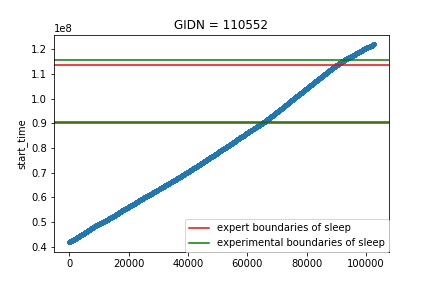
\includegraphics[width=1\linewidth]{1105521}} d) \\
	\end{minipage}
	\caption{RR-сигнал и границы найденного сна для двух людей}
	\label{ris:find_sleep_bound1}
\end{figure}
\subsubsection{Градиентный бустинг над деревьями}
Далее было принято решение увеличить количество признаков и кроме среднего и дисперсии посчитать характеристики, которые считаются информативными для работы с RR-сигналом. Здесь работа шла со следующим сигналом: RR-сигнал, последовательност RR-интервалов. Для предсказания сна RR сигнал разбивался на участки по 500 отсчетов (~5 минут). Для каждого участка подсчитывались признаки, которые потом подавались на вход алгоритму классификации.
Считали следующие признаки:

\begin{itemize}
	\item mean - среднее по всему сигналу
	\item std -дисперсия всего сигнала
	\item EBS - разница между максимальным и минимальным значения RR-сигнала
	
	Перечисленные выше признаки считались для всего сигнала. Далее идут признаки подсчитанные для каждых 500 отсчетов.
	
	\item mean window - среднее значений на 500 отсчетах
	\item std window - дисперсия на 500 отсчетах
	\item EBS window - значение EBS, посчитанное по каждым 500 отсчетам
	\item NN50 - количество двух последовательных RR-интервалов, отличающихся на 50 милисекунд
	\item pNN50 - NN50 / len(RR-сигнала)
	\item NN20 - количество двух последовательных RR-интервалов, отличающихся на 20 милисекунд
	\item pNN20 - NN20 / len(RR-сигнала)
	\item entropy - энтропия сигнала
	\item spectr entropy - спектральная энтропия
\end{itemize}
Вектор признаков, подсчитанныей для каждого 5 минутного интервала, подавался на вход классификатору. Были проведены эксперименты со случайными лесами, логистической регрессией, методом к-ближайщих.

С помощью кросс-валидации были подсчитаны ошибки для наиболее оптимальных при этой задаче параметров алгоритмов.
Наилучшее качество показал бустинг над случайными лесами:

\begin{tabular}{|c|c|c|}
	\hline \rule[-2ex]{0pt}{5.5ex} true/pred & awake & sleep \\ 
	\hline \rule[-2ex]{0pt}{5.5ex} awake & 0,85 & 0,15 \\ 
	\hline \rule[-2ex]{0pt}{5.5ex} sleep & 0,29 & 0,71 \\ 
	\hline 
	
\end{tabular}\\

Accuracy:  80\%

\subsubsection{Бустинг для предсказания пола}
Далее было принято решение увеличить количество признаков и кроме среднего и дисперсии посчитать характеристики, которые считаются информативными для работы с RR-сигналом. Здесь работа шла со следующим сигналом: RR-сигнал, последовательност RR-интервалов.
Считали следующие признаки:
\begin{itemize}
	\item mean - среднее по всему сигналу
	\item std mean - отклонение последовательности средних значений на 200 отсчетах RR сигнала от среднего по всему сигналу
	\item mean std - среднее значений дисперсии на 200 отсчетах
	\item std std - дисперсия дисперсий, посчитанных по 200 отсчетам RR-сигнала
	\item EBS - разница между максимальным и минимальным значения RR-сигнала
	\item mean EBS - среднее значение EBS, посчитанное по каждым 200 отсчетам
	\item std EBS
	\item NN50 - количество двух последовательных RR-интервалов, отличающихся на 50 милисекунд
	\item pNN50 - NN50 / len(RR-сигнала)
	\item NN20 количество двух последовательных RR-интервалов, отличающихся на 20 милисекунд
	\item pNN20 - NN20 / len(RR-сигнала)
	
	Перечислнные выше признаки подсчитывались отдельно для всего сигнала, для сигнала во время сна, для сигнала во время периода бодроствования. При анализе выделенных признаков и анализе их дальнейшей значимости было показано, что достаточно подсчитывать признаки только для всего сигнала. Качество при этом падало незначительно.
	
	\item down percentile - 5\% квантиль
	\item up percentile - 95\% квантиль
	\item entropy - энтропия сигнала
	\item spectr entropy - спектральная энтропия
	
	Предполагается, что значение RR-интервалов отличаются в периоды сна и бодровствования, и что их можно разделить на 2 кластера. Предполагаем, что RR-сигнал можно представить в виде смеси двух гаусовских распределений. Следующие признаки - оценка этой смеси. 
	
	\item gmm mean1 - математическое ожидание первого распределения
	\item gmm mean2 - математическое ожидание второго распределения
	\item gmm weight1 - процент элементов сигнала, отнесенных к первому распределени.
	\item gmm std1 - дисперсия первого распределения
	\item gmm std2 - дисперсия второго распределения
	
	Также подсчитывались геометрические характеристики сигнала
	
	\item fractal dim - фрактальная размерность
	\item hjorth dim, hjorth mobility, hjorth complexity - спектральные параметры сигнала : размерность, мощьность, изнемчивость
	\item kurtosis - четвертый момент сигнала
	\item skewness - третий момент сигнала
	\item spearmen cor 10, spearmen cor pvalue 10, spearmen cor 50, spearmen cor pvalue 50	
	,spearmen cor 100, spearmen cor pvalue 100, spearmen cor 500, spearmen cor pvalue 500 - 
	параметры кореляции Спирмена с соответствующими параметрами
%	\item angle cross - угол, под которым сходятся наглоны при подсчете значений автокореляции
\end{itemize}
Эти признаки также подавалить на вход градиентному бустингу над деревьями. 

Качество классификации пола человека - 70\%.
Качество классификации возраста человека - 65\%
\subsubsection{Предсказание сна с помощью нейросетевых методов}


Было предположено, что для адекватной работы архитектуры хватит всего 4 простых признаков: среднего и дисперсии для кадого временного отрезка, среднего и дисперсии сигнала для всего сигнала человека.

Погружение в сон - это не мгновенный процесс, поэтому необходимо каким-либо образом сохранять информацию о текущем состоянии человека и передавать ее дальше. Для решения этой задачи были использованы реккурентные нейронные сети с LSTM \cite{create_lstm} нейронами. 

Особенностью архитектуры LSTM нейрона является наличие гейта памяти, с которым можно проделывать следующие операции:
\begin{itemize}
	\item записать информацию в гейт;
	\item обнулить внутреннее состояние гейта;
	\item получить информацию из гейта.
\end{itemize}

Была реализованна следующая архитектура:

\begin{figure}[h]
	\begin{center}
		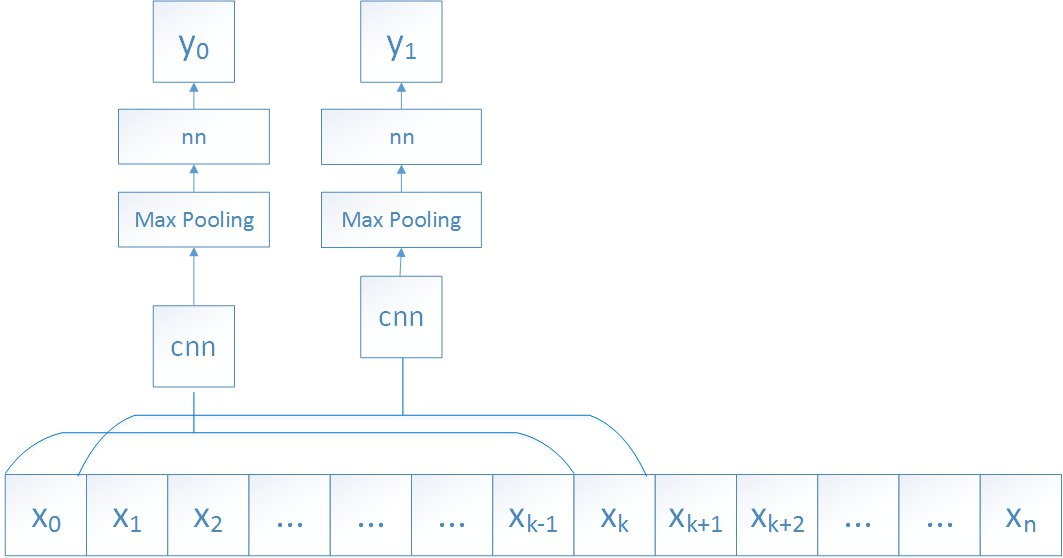
\includegraphics[scale=0.36]{arch_rnn}
		\caption{Реализованная архитектура сети}
		\label{ris:arh}
	\end{center}
\end{figure}

Для каждого 5-ти минутного интервала подсчитывались признаки $X_i$ (о них было упомянуто ранее). Далее векторов подсчитанных признаков подавался на вход реккурентному слою со 100 нейронами. Выход данного слоя подается на вход нейрону, который и выдает информацию о состоянии человека во время этого интервала. 

Были отобраны 1200 человек для обучения. Оставшиеся 600 были использованы для тестирования и валидации. 
Чтобы убедиться, что результат не зависит от отбора людей в тестовую и валидационную выборки, эксперемент был проведен несколько раз с различными случайными разбиениями.

Полученное качество (tnr == tpr) - 85\%. 

Несмотря на простоту признаков, этот метод дает лучшее качество классификации, чем предложенные ранее. 

\subsubsection{Эксперименты со сверточными сетями}

Далее встал следующий вопрос - можно ли улучшить это качество? Была предложена и реализованна следующая модель:

\begin{figure}[h]
	\begin{center}
		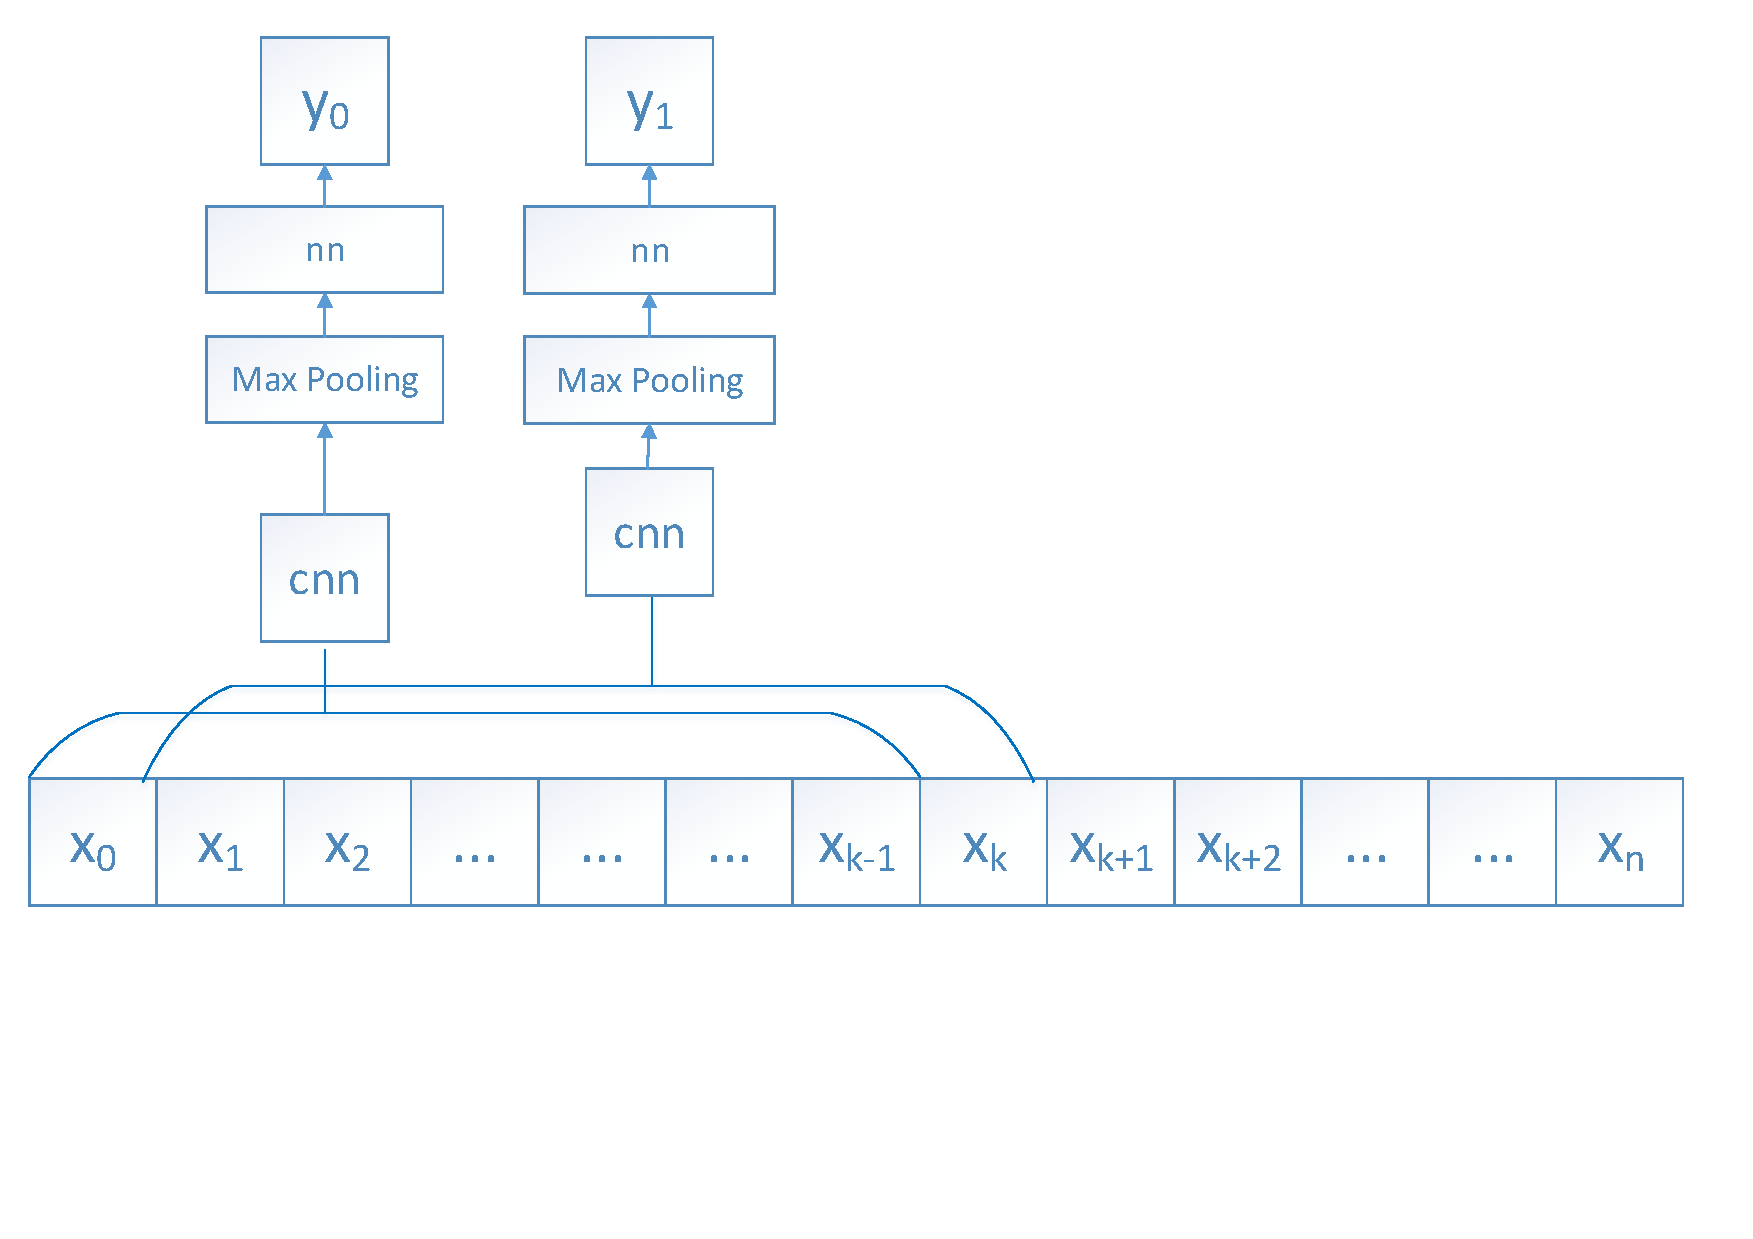
\includegraphics[scale=0.36]{arch_cnn}
		\caption{Реализованная архитектура сети}
		\label{ris:arh}
	\end{center}
\end{figure}




